% 57-79(57쪽) — 닫힌구간 [-2, 5] 에서 평균값 정리를 묻는 문항의 y=f(x) 그래프. 스캔 화질이 낮아 TikZ 로 다시 그림.
% 원문에 있는 것만: x 눈금 -2 와 5 · 그 두 곳의 세로 안내 파선 · 라벨 O, x, y, y=f(x) · 구간 밖은 파선.
% y 눈금은 원문에 없으므로 넣지 않는다(개수를 세는 문항이라 수치를 더하면 답이 드러난다).
% 곡선은 원문 모양 그대로 지나는 점들을 재서 smooth 로 잇는다(식이 주어진 그래프가 아니다).
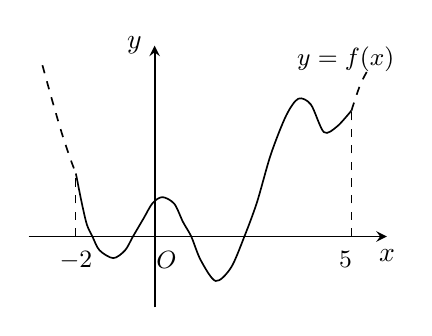
\begin{tikzpicture}[x=0.50cm, y=0.50cm, line width=0.5pt]
  \draw[->, >=stealth, line width=0.7pt] (-3.2,0) -- (5.9,0) node[below=1pt] {$x$};
  \draw[->, >=stealth, line width=0.7pt] (0,-1.8) -- (0,4.85) node[left=1pt] {$y$};
  \node[below=2pt, font=\small] at (0.3,0) {$\pt{O}$};
  % 구간 끝의 세로 안내 파선(원문)
  \draw[dashed, line width=0.35pt] (-2,0) -- (-2,1.60);
  \draw[dashed, line width=0.35pt] (5,0) -- (5,3.20);
  % 그래프 — 닫힌구간 [-2, 5] 밖은 원문처럼 파선
  \draw[dashed, line width=0.6pt, smooth] plot coordinates {(-2.85,4.35) (-2.60,3.45) (-2.35,2.60) (-2.15,2.00) (-2,1.60)};
  \draw[line width=0.6pt, smooth] plot coordinates
    {(-2,1.60) (-1.85,0.85) (-1.72,0.30) (-1.58,0) (-1.40,-0.35) (-1.05,-0.55) (-0.75,-0.35)
     (-0.55,0) (-0.28,0.46) (-0.05,0.85) (0.20,1.00) (0.50,0.83) (0.72,0.37) (0.93,0)
     (1.17,-0.60) (1.55,-1.13) (1.94,-0.79) (2.28,0) (2.60,0.87) (2.95,2.08) (3.34,3.07)
     (3.65,3.50) (3.97,3.35) (4.30,2.65) (4.64,2.80) (5,3.20)};
  \draw[dashed, line width=0.6pt, smooth] plot coordinates {(5,3.20) (5.22,3.85) (5.40,4.20)};
  \node[below=2pt, font=\small] at (-2,0) {$-2$};
  \node[below=2pt, font=\small] at (4.85,0) {$5$};
  \node[right=1pt, font=\small] at (3.3,4.5) {$y=f(x)$};
\end{tikzpicture}
